% F087｜牛顿切线法快速求近似根｜02_explanation.tex
% 继承上传模板的 LaTeX 环境；当前条目的内容独立编写。
\clearpage
\begin{explanationbox}
\textbf{\textcolor{CExplanation}{看图理解：为什么出现减法}}
\par\medskip
\begin{center}
% F087｜tangent 原创简明教学示意图
\begin{tikzpicture}[>=stealth,scale=.82]
\draw[->] (0,0)--(7.6,0) node[right]{$x$};\draw[->] (.8,-1.4)--(.8,3.2) node[above]{$y$};
% 横向比例尺 x_point=8(x-2.65)，纵向比例尺 y_point=0.75(x^2-10)。
\draw[teal,thick,domain=2.76:3.48,samples=45] plot ({8*(\x-2.65)},{.75*(\x*\x-10)});
% 在真实点 x_0=3 的切线；交轴位置 x_1=19/6。
\draw[orange,thick] (2,-1.2)--(6,1.05);
\fill[orange] (2.8,-.75) circle (2pt) node[below left=5pt]{$x_0=3$};
\fill[orange] (4.1333,0) circle(2pt) node[below=7pt]{$x_1\approx3.1667$};
\node at (5.5,2.7){\small 用切线寻找新的交点};
\node[teal] at (5.7,1.9){\small $y=x^2-10$};
\end{tikzpicture}

\end{center}
\medskip
在 $(x_n,f(x_n))$ 点作切线。若切线斜率为 $k$，向横轴移动时纵坐标要从 $f(x_n)$ 变为 $0$，横向需要移动 $-f(x_n)/k$，因此新横坐标是 $x_n-f(x_n)/k$。
\end{explanationbox}
\clearpage
\begin{explanationbox}
\textbf{\textcolor{CExplanation}{平方根为什么是“取平均”}}
\par\medskip
\begin{center}
% F087｜square 原创简明教学示意图
\begin{tikzpicture}[>=stealth,scale=.9]
\node[draw,fill=teal!8,rounded corners,minimum width=7.3cm,minimum height=1.5cm,align=center] at (4,0) {$x_{n+1}=\dfrac12\left(x_n+\dfrac{A}{x_n}\right)$};
\node at (4,-1.2) {\small 正数 $x_n$ 与 $A/x_n$ 的平均数};
\end{tikzpicture}

\end{center}
\medskip
用 $f(x)=x^2-A$，切线斜率 $f'(x)=2x$。\[x_{n+1}=x_n-\frac{x_n^2-A}{2x_n}=\frac12\left(x_n+\frac A{x_n}\right).\]如果猜得偏大，$A/x_n$ 会偏小；取两者平均就能调整。
\end{explanationbox}
\clearpage
\begin{explanationbox}
\textbf{\textcolor{CExplanation}{什么时候不该盲用}}
\par\medskip
\begin{center}
% F087｜steps 原创简明教学示意图
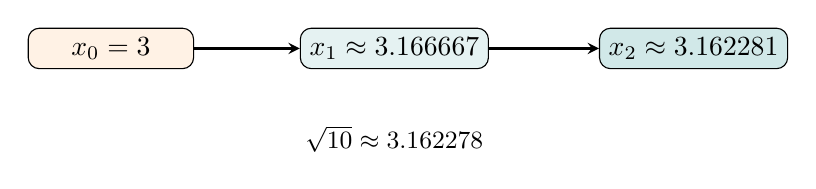
\begin{tikzpicture}[>=stealth,node distance=1cm]
\node[draw,rounded corners,fill=orange!10,minimum width=2.1cm] (a) at (0,0) {$x_0=3$};
\node[draw,rounded corners,fill=teal!10,minimum width=2.3cm] (b) at (3.6,0) {$x_1\approx3.166667$};
\node[draw,rounded corners,fill=teal!18,minimum width=2.3cm] (c) at (7.4,0) {$x_2\approx3.162281$};
\draw[->,thick] (a)--(b);\draw[->,thick] (b)--(c);
\node at (3.6,-1.15) {\small $\sqrt{10}\approx3.162278$};
\end{tikzpicture}

\end{center}
\medskip
切线可能几乎水平，也可能把新点推向很远处。只有在函数足够平滑、初值选得合适时，连续更新才会有效。对一个具体问题，算完应将结果代回原方程检验。
\end{explanationbox}
